\documentclass[a4paper,10pt]{article}
\usepackage{graphicx,color}
\usepackage[margin=2cm]{geometry}
\usepackage{algorithm2e}

\begin{document}

{\LARGE{\centerline{\bf Lab 1}}}
\Large{Brendon Swanepoel - 601949, Anita de Mello Koch - 1371116, \\ Nicholas Kastanos - 1440624}

\section{3-D Array Multiplication}

To obtain each element in matrix $C$, matrix $A$ and $B$ are divided into two-dimensional matrices, $A'$ and $B'$ as can be seen in figure \ref{3DMult}.
For each two-dimensional matrix, a single row and column is multiplied to get the corresponding element in the $C$ matrix.
This leads to a single value which is the element in the $C$ matrix.
This is done for all elements in the $C$ matrix.

\begin{figure}[h]
\centering
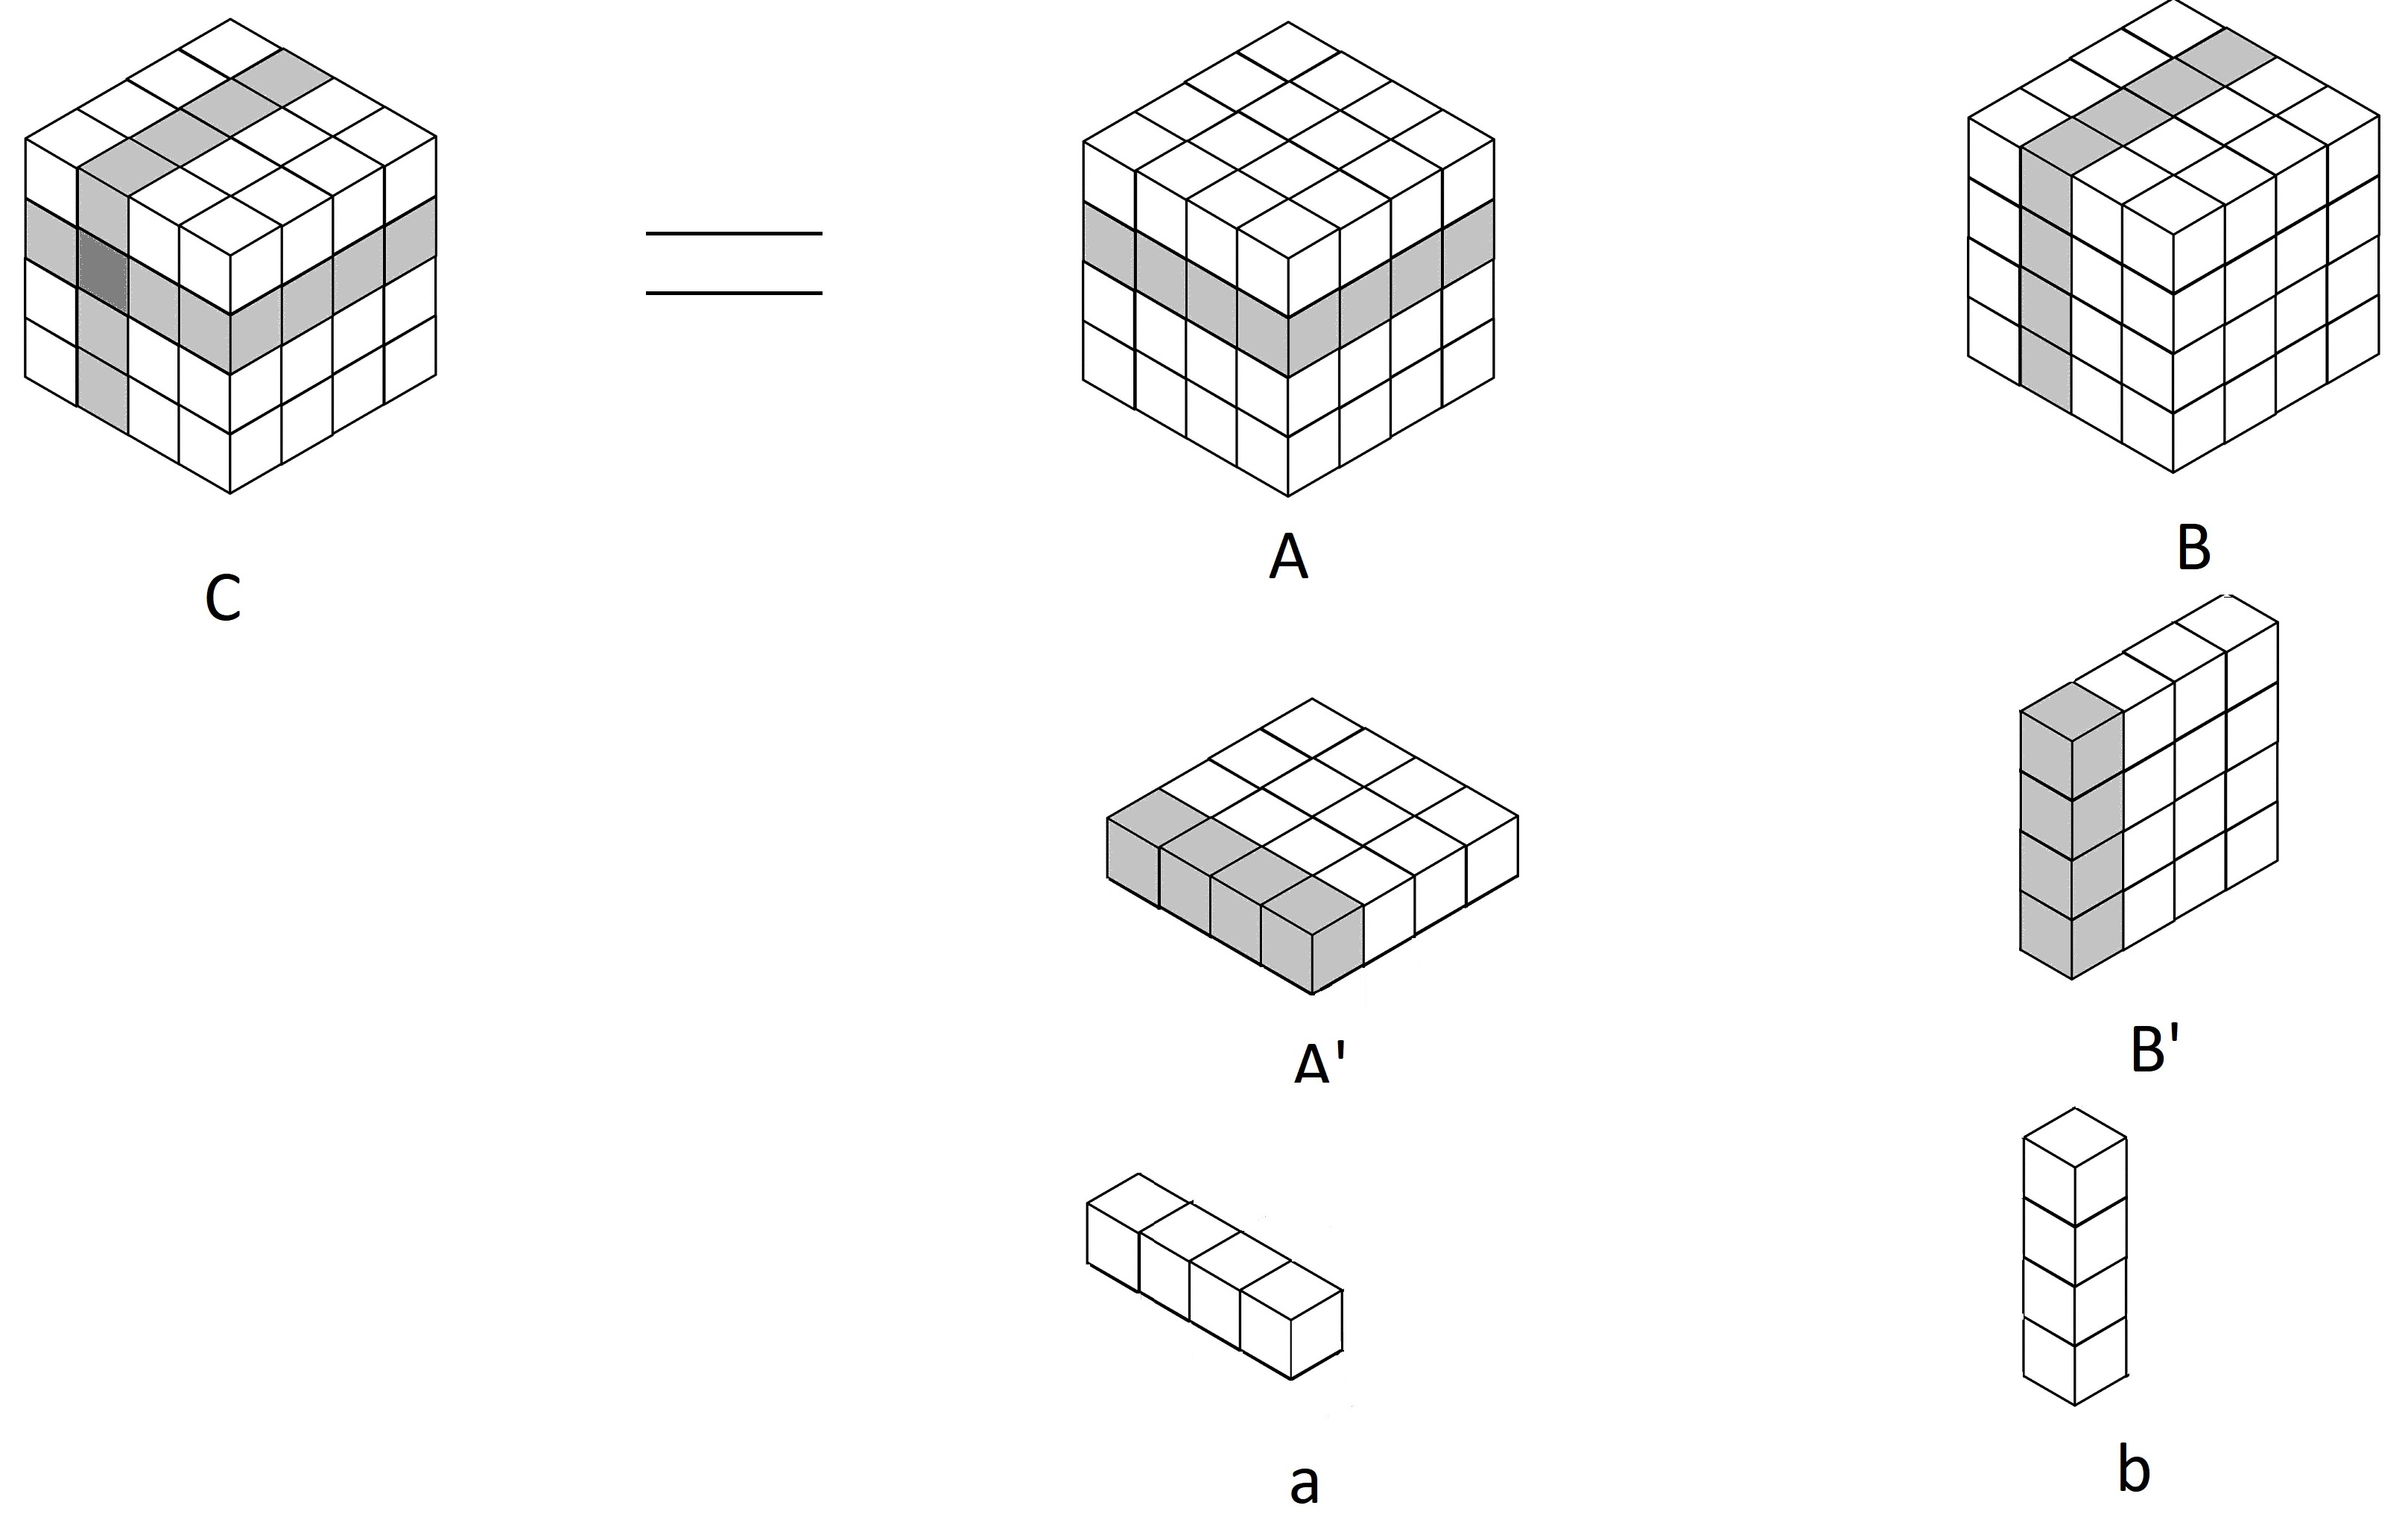
\includegraphics[scale=0.15]{3D.jpg}
\caption{How each element in $C$ was obtained from matrices $A$ and $B$.}\label{3DMult}
\end{figure}

Two \texttt{for} loops were used to maintain the row and column of the current element in matrix $C$.
Another \texttt{for} loop was used to traverse the depth of the matrix $C$.
The row $a$ and column $b$ were then obtained from matrices $A$ and $B$ as seen in figure \ref{3DMult}.
Vector multiplication was then used on vectors $a$ and $b$.
The resulting value is the corresponding element of $C$.

This was repeated for all elements in matrix $C$.
It was assumed matrix $A$ and $B$ are cubes.

\section{Generalizing for $N$ dimensions}

To multiply a multi-dimensional array of $N$ dimensions, a recursive function can be used.

This can be done by inputting the two $N$ dimensional arrays and the value $N$.
For the two, multi-dimensional arrays, extract a single plane and call the function on these $N-1$ multi-dimensional arrays.
This process is continued until a single vector remains from each matrix.
The vector product of these two vectors is the result of the corresponding element in the resultant $N$ multi-dimensional array.

\section{Pseudocode}

\begin{algorithm}[H]
	\SetAlgoLined
	\SetKwData{Left}{left}\SetKwData{This}{this}\SetKwData{Up}{up}
	\SetKwFunction{Union}{Union}\SetKwFunction{FindCompress}{FindCompress}
	\SetKwInOut{Input}{input}\SetKwInOut{Output}{output}
	\Input{Two 2D square matrices}
	\Output{Calculating the addition of two 2D square matrices}
	initialise results matrix\; 
	\For{Each row of the matrix}{
		\For{Each column element in the current row}{
			Sum the corresponding row and column elements of\\
			both matrices\;
			Store sum value in result matrix\;
		}
	}

	Return results matrix\;
\caption{2D Addition Algorithm}
\end{algorithm}

\begin{algorithm}[H]
	\SetAlgoLined
	\SetKwData{Left}{left}\SetKwData{This}{this}\SetKwData{Up}{up}
	\SetKwFunction{Union}{Union}\SetKwFunction{FindCompress}{FindCompress}
	\SetKwInOut{Input}{input}\SetKwInOut{Output}{output}
	\Input{Two 3D cubic matrices}
	\Output{Calculating the addition of two 3D cubic matrices}
	initialise results matrix\;
	\For{Each depth row of the cube}{
		\For{Each row of the cube at the current depth}{
			\For{Each column element at the current depth and row}{
				Sum the corresponding row and column elements of\\ 
				both matrices at the current depth\;
				Store sum value in result matrix\;
			}
		}
	}
	Return results matrix\;
	\caption{3D Addition Algorithm}
\end{algorithm}


\begin{algorithm}[H]
	\SetAlgoLined
	\SetKwData{Left}{left}\SetKwData{This}{this}\SetKwData{Up}{up}
	\SetKwFunction{Union}{Union}\SetKwFunction{FindCompress}{FindCompress}
	\SetKwInOut{Input}{input}\SetKwInOut{Output}{output}
	\Input{Two 2D square matricesB}
	\Output{Calculating the multiplication of two 2D square matrices}
	initialise results matrix\;
	\For{Each row of the square}{
		\For{Each column of the square at the current row}{
			\For{Each element in the row and column of the corresponding matrices}{
				Mutiply and sum the corresponding row and column elements\;
			}
			Store sum value in result matrix\;
		}
	}
	Return results matrix\;
	\caption{2D Multiplication Algorithm}
	
\end{algorithm}

\begin{algorithm}[H]
\SetAlgoLined
\SetKwData{Left}{left}\SetKwData{This}{this}\SetKwData{Up}{up}
\SetKwFunction{Union}{Union}\SetKwFunction{FindCompress}{FindCompress}
\SetKwInOut{Input}{input}\SetKwInOut{Output}{output}
\Input{Matrix A and B, two 3D cubic matrices}
\Output{Matrix C, the multiple of two 3D matrices}
\BlankLine
\For{each row in matrix C}{
\For{each column in matrix C}{\label{forins}
\For{each depth in matrix C}{
Get corresponding row at depth from matrix A\;
Get corresponding column at depth from matrix B\;
Multiply the obtained row and column to get the value of matrix C at the current row, column and depth.
}}}
\caption{3D Multiplication Algorithm}\label{algo_disjdecomp}

\end{algorithm}

\end{document}